%% bare_jrnl.tex
%% V1.4b
%% 2015/08/26
%% by Michael Shell
%% see http://www.michaelshell.org/
%% for current contact information.
%%
%% This is a skeleton file demonstrating the use of IEEEtran.cls
%% (requires IEEEtran.cls version 1.8b or later) with an IEEE
%% journal paper.
%%
%% Support sites:
%% http://www.michaelshell.org/tex/ieeetran/
%% http://www.ctan.org/pkg/ieeetran
%% and
%% http://www.ieee.org/

%%*************************************************************************
%% Legal Notice:
%% This code is offered as-is without any warranty either expressed or
%% implied; without even the implied warranty of MERCHANTABILITY or
%% FITNESS FOR A PARTICULAR PURPOSE! 
%% User assumes all risk.
%% In no event shall the IEEE or any contributor to this code be liable for
%% any damages or losses, including, but not limited to, incidental,
%% consequential, or any other damages, resulting from the use or misuse
%% of any information contained here.
%%
%% All comments are the opinions of their respective authors and are not
%% necessarily endorsed by the IEEE.
%%
%% This work is distributed under the LaTeX Project Public License (LPPL)
%% ( http://www.latex-project.org/ ) version 1.3, and may be freely used,
%% distributed and modified. A copy of the LPPL, version 1.3, is included
%% in the base LaTeX documentation of all distributions of LaTeX released
%% 2003/12/01 or later.
%% Retain all contribution notices and credits.
%% ** Modified files should be clearly indicated as such, including  **
%% ** renaming them and changing author support contact information. **
%%*************************************************************************


% *** Authors should verify (and, if needed, correct) their LaTeX system  ***
% *** with the testflow diagnostic prior to trusting their LaTeX platform ***
% *** with production work. The IEEE's font choices and paper sizes can   ***
% *** trigger bugs that do not appear when using other class files.       ***                          ***
% The testflow support page is at:
% http://www.michaelshell.org/tex/testflow/



\documentclass[journal]{IEEEtran}
%
% If IEEEtran.cls has not been installed into the LaTeX system files,
% manually specify the path to it like:
% \documentclass[journal]{../sty/IEEEtran}





% Some very useful LaTeX packages include:
% (uncomment the ones you want to load)
\usepackage[acronym]{glossaries}

\newacronym[]{ir}{IR}{Infrared}
\newacronym[]{fov}{FOV}{Field of View}
\newacronym[]{sad}{SAD}{Sum of Absolute Differences}
\newacronym[]{lut}{LUT}{Look Up Table}
\newacronym[]{cmos}{CMOS}{Complementary metal–oxide–semiconductor}
\newacronym[]{dof}{DOF}{Depth of field}

% *** MISC UTILITY PACKAGES ***
%
%\usepackage{ifpdf}
% Heiko Oberdiek's ifpdf.sty is very useful if you need conditional
% compilation based on whether the output is pdf or dvi.
% usage:
% \ifpdf
%   % pdf code
% \else
%   % dvi code
% \fi
% The latest version of ifpdf.sty can be obtained from:
% http://www.ctan.org/pkg/ifpdf
% Also, note that IEEEtran.cls V1.7 and later provides a builtin
% \ifCLASSINFOpdf conditional that works the same way.
% When switching from latex to pdflatex and vice-versa, the compiler may
% have to be run twice to clear warning/error messages.






% *** CITATION PACKAGES ***
%
\usepackage{cite}
% cite.sty was written by Donald Arseneau
% V1.6 and later of IEEEtran pre-defines the format of the cite.sty package
% \cite{} output to follow that of the IEEE. Loading the cite package will
% result in citation numbers being automatically sorted and properly
% "compressed/ranged". e.g., [1], [9], [2], [7], [5], [6] without using
% cite.sty will become [1], [2], [5]--[7], [9] using cite.sty. cite.sty's
% \cite will automatically add leading space, if needed. Use cite.sty's
% noadjust option (cite.sty V3.8 and later) if you want to turn this off
% such as if a citation ever needs to be enclosed in parenthesis.
% cite.sty is already installed on most LaTeX systems. Be sure and use
% version 5.0 (2009-03-20) and later if using hyperref.sty.
% The latest version can be obtained at:
% http://www.ctan.org/pkg/cite
% The documentation is contained in the cite.sty file itself.






% *** GRAPHICS RELATED PACKAGES ***
%
\ifCLASSINFOpdf
   \usepackage[pdftex]{graphicx}
  % declare the path(s) where your graphic files are
  % \graphicspath{{../pdf/}{../jpeg/}}
  % and their extensions so you won't have to specify these with
  % every instance of \includegraphics
  % \DeclareGraphicsExtensions{.pdf,.jpeg,.png}
\else
  % or other class option (dvipsone, dvipdf, if not using dvips). graphicx
  % will default to the driver specified in the system graphics.cfg if no
  % driver is specified.
  % \usepackage[dvips]{graphicx}
  % declare the path(s) where your graphic files are
  % \graphicspath{{../eps/}}
  % and their extensions so you won't have to specify these with
  % every instance of \includegraphics
  % \DeclareGraphicsExtensions{.eps}
\fi
% graphicx was written by David Carlisle and Sebastian Rahtz. It is
% required if you want graphics, photos, etc. graphicx.sty is already
% installed on most LaTeX systems. The latest version and documentation
% can be obtained at: 
% http://www.ctan.org/pkg/graphicx
% Another good source of documentation is "Using Imported Graphics in
% LaTeX2e" by Keith Reckdahl which can be found at:
% http://www.ctan.org/pkg/epslatex
%
% latex, and pdflatex in dvi mode, support graphics in encapsulated
% postscript (.eps) format. pdflatex in pdf mode supports graphics
% in .pdf, .jpeg, .png and .mps (metapost) formats. Users should ensure
% that all non-photo figures use a vector format (.eps, .pdf, .mps) and
% not a bitmapped formats (.jpeg, .png). The IEEE frowns on bitmapped formats
% which can result in "jaggedy"/blurry rendering of lines and letters as
% well as large increases in file sizes.
%
% You can find documentation about the pdfTeX application at:
% http://www.tug.org/applications/pdftex





% *** MATH PACKAGES ***
%
%\usepackage{amsmath}
% A popular package from the American Mathematical Society that provides
% many useful and powerful commands for dealing with mathematics.
%
% Note that the amsmath package sets \interdisplaylinepenalty to 10000
% thus preventing page breaks from occurring within multiline equations. Use:
%\interdisplaylinepenalty=2500
% after loading amsmath to restore such page breaks as IEEEtran.cls normally
% does. amsmath.sty is already installed on most LaTeX systems. The latest
% version and documentation can be obtained at:
% http://www.ctan.org/pkg/amsmath





% *** SPECIALIZED LIST PACKAGES ***
%
%\usepackage{algorithmic}
% algorithmic.sty was written by Peter Williams and Rogerio Brito.
% This package provides an algorithmic environment fo describing algorithms.
% You can use the algorithmic environment in-text or within a figure
% environment to provide for a floating algorithm. Do NOT use the algorithm
% floating environment provided by algorithm.sty (by the same authors) or
% algorithm2e.sty (by Christophe Fiorio) as the IEEE does not use dedicated
% algorithm float types and packages that provide these will not provide
% correct IEEE style captions. The latest version and documentation of
% algorithmic.sty can be obtained at:
% http://www.ctan.org/pkg/algorithms
% Also of interest may be the (relatively newer and more customizable)
% algorithmicx.sty package by Szasz Janos:
% http://www.ctan.org/pkg/algorithmicx




% *** ALIGNMENT PACKAGES ***
%
%\usepackage{array}
% Frank Mittelbach's and David Carlisle's array.sty patches and improves
% the standard LaTeX2e array and tabular environments to provide better
% appearance and additional user controls. As the default LaTeX2e table
% generation code is lacking to the point of almost being broken with
% respect to the quality of the end results, all users are strongly
% advised to use an enhanced (at the very least that provided by array.sty)
% set of table tools. array.sty is already installed on most systems. The
% latest version and documentation can be obtained at:
% http://www.ctan.org/pkg/array


% IEEEtran contains the IEEEeqnarray family of commands that can be used to
% generate multiline equations as well as matrices, tables, etc., of high
% quality.




% *** SUBFIGURE PACKAGES ***
\usepackage{placeins}
\ifCLASSOPTIONcompsoc
 \usepackage[caption=false,font=normalsize,labelfont=sf,textfont=sf]{subfig}
\else
 \usepackage[caption=false,font=footnotesize]{subfig}
\fi
% subfig.sty, written by Steven Douglas Cochran, is the modern replacement
% for subfigure.sty, the latter of which is no longer maintained and is
% incompatible with some LaTeX packages including fixltx2e. However,
% subfig.sty requires and automatically loads Axel Sommerfeldt's caption.sty
% which will override IEEEtran.cls' handling of captions and this will result
% in non-IEEE style figure/table captions. To prevent this problem, be sure
% and invoke subfig.sty's "caption=false" package option (available since
% subfig.sty version 1.3, 2005/06/28) as this is will preserve IEEEtran.cls
% handling of captions.
% Note that the Computer Society format requires a larger sans serif font
% than the serif footnote size font used in traditional IEEE formatting
% and thus the need to invoke different subfig.sty package options depending
% on whether compsoc mode has been enabled.
%
% The latest version and documentation of subfig.sty can be obtained at:
% http://www.ctan.org/pkg/subfig




% *** FLOAT PACKAGES ***
%
%\usepackage{fixltx2e}
% fixltx2e, the successor to the earlier fix2col.sty, was written by
% Frank Mittelbach and David Carlisle. This package corrects a few problems
% in the LaTeX2e kernel, the most notable of which is that in current
% LaTeX2e releases, the ordering of single and double column floats is not
% guaranteed to be preserved. Thus, an unpatched LaTeX2e can allow a
% single column figure to be placed prior to an earlier double column
% figure.
% Be aware that LaTeX2e kernels dated 2015 and later have fixltx2e.sty's
% corrections already built into the system in which case a warning will
% be issued if an attempt is made to load fixltx2e.sty as it is no longer
% needed.
% The latest version and documentation can be found at:
% http://www.ctan.org/pkg/fixltx2e


%\usepackage{stfloats}
% stfloats.sty was written by Sigitas Tolusis. This package gives LaTeX2e
% the ability to do double column floats at the bottom of the page as well
% as the top. (e.g., "\begin{figure*}[!b]" is not normally possible in
% LaTeX2e). It also provides a command:
%\fnbelowfloat
% to enable the placement of footnotes below bottom floats (the standard
% LaTeX2e kernel puts them above bottom floats). This is an invasive package
% which rewrites many portions of the LaTeX2e float routines. It may not work
% with other packages that modify the LaTeX2e float routines. The latest
% version and documentation can be obtained at:
% http://www.ctan.org/pkg/stfloats
% Do not use the stfloats baselinefloat ability as the IEEE does not allow
% \baselineskip to stretch. Authors submitting work to the IEEE should note
% that the IEEE rarely uses double column equations and that authors should try
% to avoid such use. Do not be tempted to use the cuted.sty or midfloat.sty
% packages (also by Sigitas Tolusis) as the IEEE does not format its papers in
% such ways.
% Do not attempt to use stfloats with fixltx2e as they are incompatible.
% Instead, use Morten Hogholm'a dblfloatfix which combines the features
% of both fixltx2e and stfloats:
%
% \usepackage{dblfloatfix}
% The latest version can be found at:
% http://www.ctan.org/pkg/dblfloatfix




%\ifCLASSOPTIONcaptionsoff
%  \usepackage[nomarkers]{endfloat}
% \let\MYoriglatexcaption\caption
% \renewcommand{\caption}[2][\relax]{\MYoriglatexcaption[#2]{#2}}
%\fi
% endfloat.sty was written by James Darrell McCauley, Jeff Goldberg and 
% Axel Sommerfeldt. This package may be useful when used in conjunction with 
% IEEEtran.cls'  captionsoff option. Some IEEE journals/societies require that
% submissions have lists of figures/tables at the end of the paper and that
% figures/tables without any captions are placed on a page by themselves at
% the end of the document. If needed, the draftcls IEEEtran class option or
% \CLASSINPUTbaselinestretch interface can be used to increase the line
% spacing as well. Be sure and use the nomarkers option of endfloat to
% prevent endfloat from "marking" where the figures would have been placed
% in the text. The two hack lines of code above are a slight modification of
% that suggested by in the endfloat docs (section 8.4.1) to ensure that
% the full captions always appear in the list of figures/tables - even if
% the user used the short optional argument of \caption[]{}.
% IEEE papers do not typically make use of \caption[]'s optional argument,
% so this should not be an issue. A similar trick can be used to disable
% captions of packages such as subfig.sty that lack options to turn off
% the subcaptions:
% For subfig.sty:
% \let\MYorigsubfloat\subfloat
% \renewcommand{\subfloat}[2][\relax]{\MYorigsubfloat[]{#2}}
% However, the above trick will not work if both optional arguments of
% the \subfloat command are used. Furthermore, there needs to be a
% description of each subfigure *somewhere* and endfloat does not add
% subfigure captions to its list of figures. Thus, the best approach is to
% avoid the use of subfigure captions (many IEEE journals avoid them anyway)
% and instead reference/explain all the subfigures within the main caption.
% The latest version of endfloat.sty and its documentation can obtained at:
% http://www.ctan.org/pkg/endfloat
%
% The IEEEtran \ifCLASSOPTIONcaptionsoff conditional can also be used
% later in the document, say, to conditionally put the References on a 
% page by themselves.




% *** PDF, URL AND HYPERLINK PACKAGES ***
%
\usepackage{url}
% url.sty was written by Donald Arseneau. It provides better support for
% handling and breaking URLs. url.sty is already installed on most LaTeX
% systems. The latest version and documentation can be obtained at:
% http://www.ctan.org/pkg/url
% Basically, \url{my_url_here}.




% *** Do not adjust lengths that control margins, column widths, etc. ***
% *** Do not use packages that alter fonts (such as pslatex).         ***
% There should be no need to do such things with IEEEtran.cls V1.6 and later.
% (Unless specifically asked to do so by the journal or conference you plan
% to submit to, of course. )


% correct bad hyphenation here
\hyphenation{op-tical net-works semi-conduc-tor}


\begin{document}
%
% paper title
% Titles are generally capitalized except for words such as a, an, and, as,
% at, but, by, for, in, nor, of, on, or, the, to and up, which are usually
% not capitalized unless they are the first or last word of the title.
% Linebreaks \\ can be used within to get better formatting as desired.
% Do not put math or special symbols in the title.
\title{3D structured light reconstruction system}
%
%
% author names and IEEE memberships
% note positions of commas and nonbreaking spaces ( ~ ) LaTeX will not break
% a structure at a ~ so this keeps an author's name from being broken across
% two lines.
% use \thanks{} to gain access to the first footnote area
% a separate \thanks must be used for each paragraph as LaTeX2e's \thanks
% was not built to handle multiple paragraphs
%

\author{João~Santos~76912,~\IEEEmembership{DETI UA,}
        Samuel~Silva~93428,~\IEEEmembership{DETI UA}}% <-this % stops a space
% \thanks{M. Shell was with the Department
% of Electrical and Computer Engineering, Georgia Institute of Technology, Atlanta,
% GA, 30332 USA e-mail: (see http://www.michaelshell.org/contact.html).}% <-this % stops a space
% \thanks{J. Doe and J. Doe are with Anonymous University.}% <-this % stops a space}

% note the % following the last \IEEEmembership and also \thanks - 
% these prevent an unwanted space from occurring between the last author name
% and the end of the author line. i.e., if you had this:
% 
% \author{....lastname \thanks{...} \thanks{...} }
%                     ^------------^------------^----Do not want these spaces!
%
% a space would be appended to the last name and could cause every name on that
% line to be shifted left slightly. This is one of those "LaTeX things". For
% instance, "\textbf{A} \textbf{B}" will typeset as "A B" not "AB". To get
% "AB" then you have to do: "\textbf{A}\textbf{B}"
% \thanks is no different in this regard, so shield the last } of each \thanks
% that ends a line with a % and do not let a space in before the next \thanks.
% Spaces after \IEEEmembership other than the last one are OK (and needed) as
% you are supposed to have spaces between the names. For what it is worth,
% this is a minor point as most people would not even notice if the said evil
% space somehow managed to creep in.



% The paper headers
\markboth{Computer Vision, 2021-2022, DETI UA}%
{Shell \MakeLowercase{\textit{et al.}}: Bare Demo of IEEEtran.cls for IEEE Journals}
% The only time the second header will appear is for the odd numbered pages
% after the title page when using the twoside option.
% 
% *** Note that you probably will NOT want to include the author's ***
% *** name in the headers of peer review papers.                   ***
% You can use \ifCLASSOPTIONpeerreview for conditional compilation here if
% you desire.




% If you want to put a publisher's ID mark on the page you can do it like
% this:
%\IEEEpubid{0000--0000/00\$00.00~\copyright~2015 IEEE}
% Remember, if you use this you must call \IEEEpubidadjcol in the second
% column for its text to clear the IEEEpubid mark.



% use for special paper notices
%\IEEEspecialpapernotice{(Invited Paper)}




% make the title area
\maketitle

% As a general rule, do not put math, special symbols or citations
% in the abstract or keywords.
\begin{abstract}
TODO
\end{abstract}

% Note that keywords are not normally used for peerreview papers.
\begin{IEEEkeywords}
Infrared, dot pattern, Kinect, speckle, structured light, point cloud
\end{IEEEkeywords}






% For peer review papers, you can put extra information on the cover
% page as needed:
% \ifCLASSOPTIONpeerreview
% \begin{center} \bfseries EDICS Category: 3-BBND \end{center}
% \fi
%
% For peerreview papers, this IEEEtran command inserts a page break and
% creates the second title. It will be ignored for other modes.
\IEEEpeerreviewmaketitle



\section{Introduction}
% The very first letter is a 2 line initial drop letter followed
% by the rest of the first word in caps.
% 
% form to use if the first word consists of a single letter:
% \IEEEPARstart{A}{demo} file is ....
% 
% form to use if you need the single drop letter followed by
% normal text (unknown if ever used by the IEEE):
% \IEEEPARstart{A}{}demo file is ....
% 
% Some journals put the first two words in caps:
% \IEEEPARstart{T}{his demo} file is ....
% 
% Here we have the typical use of a "T" for an initial drop letter
% and "HIS" in caps to complete the first word.
\IEEEPARstart{T}{he} Xbox 360 Kinect has opened a new era of inexpensive 3D sensing. It was originally intended only for the gaming industry, but it was quickly adopted by scientists, robotics enthusiasts, and hobbyists all over the world. This sensor was introduced as a low-cost, durable, marker-free, and reliable device capable of recording real-time proximity and depth data. It combines a standard color camera with a depth camera that incorporates an \gls{ir} laser projector as well as an  \gls{ir} camera. The Windows Software Development Kit (SDK) 2.0 has enabled the development of software that use the gesture recognition technology built in the device to integrate joint orientation and skeleton tracking for joint positions in standing and seated positions, among many other applications.

In the scope of this work, we will study and replicate the depth estimation algorithm that is suspected to be implemented on the Kinect system. To achieve so, firstly a set of simulated \gls{ir} images will be the input for the depth estimation. As a final goal, a real Kinect was intended to be used solely for the projection and detection of the speckle pattern, to then process it into the desired point cloud format.



% o mundo à nossa volta é todo ele em 3 dimensões. No entanto, até mesmo as camaras mais sofisticadas não têm a perceção de profundidade, passando assim, tudo o que capturam para uma imagem a 2 dimensões. Desta forma, características importantes como a profundidade, as distâncias e os ângulos não são preservados. Para além disso as camaras introduzem distorção. Com este relatório, através de luz estruturada, pretende-se recriar um objeto sem perder as características do mundo real. Para recriar um objeto através de luz estruturada são necessários dois componentes: um projetor que emite um padrão sobre o objeto a recriar; numa câmara que recolhe a imagem gerada. O objeto vai criar uma distorção no padrão original e é com base na distorção do padrão que vai ser construída uma imagem de disparidade para posteriormente reconstruir o objeto.  

% You must have at least 2 lines in the paragraph with the drop letter
% (should never be an issue)


% needed in second column of first page if using \IEEEpubid
%\IEEEpubidadjcol




% An example of a floating figure using the graphicx package.
% Note that \label must occur AFTER (or within) \caption.
% For figures, \caption should occur after the \includegraphics.
% Note that IEEEtran v1.7 and later has special internal code that
% is designed to preserve the operation of \label within \caption
% even when the captionsoff option is in effect. However, because
% of issues like this, it may be the safest practice to put all your
% \label just after \caption rather than within \caption{}.
%
% Reminder: the "draftcls" or "draftclsnofoot", not "draft", class
% option should be used if it is desired that the figures are to be
% displayed while in draft mode.
%
%\begin{figure}[!t]
%\centering
%\includegraphics[width=2.5in]{myfigure}
% where an .eps filename suffix will be assumed under latex, 
% and a .pdf suffix will be assumed for pdflatex; or what has been declared
% via \DeclareGraphicsExtensions.
%\caption{Simulation results for the network.}
%\label{fig_sim}
%\end{figure}

% Note that the IEEE typically puts floats only at the top, even when this
% results in a large percentage of a column being occupied by floats.


% An example of a double column floating figure using two subfigures.
% (The subfig.sty package must be loaded for this to work.)
% The subfigure \label commands are set within each subfloat command,
% and the \label for the overall figure must come after \caption.
% \hfil is used as a separator to get equal spacing.
% Watch out that the combined width of all the subfigures on a 
% line do not exceed the text width or a line break will occur.
%
%\begin{figure*}[!t]
%\centering
%\subfloat[Case I]{\includegraphics[width=2.5in]{box}%
%\label{fig_first_case}}
%\hfil
%\subfloat[Case II]{\includegraphics[width=2.5in]{box}%
%\label{fig_second_case}}
%\caption{Simulation results for the network.}
%\label{fig_sim}
%\end{figure*}
%
% Note that often IEEE papers with subfigures do not employ subfigure
% captions (using the optional argument to \subfloat[]), but instead will
% reference/describe all of them (a), (b), etc., within the main caption.
% Be aware that for subfig.sty to generate the (a), (b), etc., subfigure
% labels, the optional argument to \subfloat must be present. If a
% subcaption is not desired, just leave its contents blank,
% e.g., \subfloat[].


% An example of a floating table. Note that, for IEEE style tables, the
% \caption command should come BEFORE the table and, given that table
% captions serve much like titles, are usually capitalized except for words
% such as a, an, and, as, at, but, by, for, in, nor, of, on, or, the, to
% and up, which are usually not capitalized unless they are the first or
% last word of the caption. Table text will default to \footnotesize as
% the IEEE normally uses this smaller font for tables.
% The \label must come after \caption as always.
%
%\begin{table}[!t]
%% increase table row spacing, adjust to taste
%\renewcommand{\arraystretch}{1.3}
% if using array.sty, it might be a good idea to tweak the value of
% \extrarowheight as needed to properly center the text within the cells
%\caption{An Example of a Table}
%\label{table_example}
%\centering
%% Some packages, such as MDW tools, offer better commands for making tables
%% than the plain LaTeX2e tabular which is used here.
%\begin{tabular}{|c||c|}
%\hline
%One & Two\\
%\hline
%Three & Four\\
%\hline
%\end{tabular}
%\end{table}


% Note that the IEEE does not put floats in the very first column
% - or typically anywhere on the first page for that matter. Also,
% in-text middle ("here") positioning is typically not used, but it
% is allowed and encouraged for Computer Society conferences (but
% not Computer Society journals). Most IEEE journals/conferences use
% top floats exclusively. 
% Note that, LaTeX2e, unlike IEEE journals/conferences, places
% footnotes above bottom floats. This can be corrected via the
% \fnbelowfloat command of the stfloats package.

\section{Kinect Model}

Accordingly to \cite{landau2016kinect}, as soon as the Kinect gathers an image of the projected speckle \gls{ir} pattern, this image is thresholded to then start the disparity estimation step. 

The Kinect depth system is constituted by a class 1M \gls{ir} laser (called transmitter) and a \gls{cmos} sensor (called receiver). Both transmitter and receiver are coplanar and positioned so that their optical axes are parallel and have a baseline distance of 75 mm apart. This baseline $b=75$ distance is a crucial parameter in the depth estimation since it appears on the triangulation equation \ref{eq:stereo-triangulation} (where $f_x$ is the horizontal focal distance and $d$ is the disparity value of a given pixel).

\begin{equation}
    z = f_x \frac{b}{d}
    \label{eq:stereo-triangulation}
\end{equation}

To compute the also necessary $x$ and $y$ coordinates, one uses equations \ref{eq:pointcloud_x} and \ref{eq:pointcloud_y} in which $c_x$ and $c_y$ are the skew values from the intrinsic calibration, $u$ and $v$ are the pixel coordinates of the pixel and $f_y$ is the vertical focal distance.

\begin{align} 
x &= (u - c_x) \times \frac{z}{f_x} \label{eq:pointcloud_x} \\ 
y &= (v - c_y) \times \frac{z}{f_y} \label{eq:pointcloud_y}
\end{align}

Notice that the thresholding algorithm is assumed to be implemented on the Kinect always outputs any given dot on the pattern as a single white pixel.

\subsection{Disparity Estimation}

The disparity estimation performed by the Kinect is based on a local, pixel-based correlation algorithm in which a $9\times9$ window of the mentioned binary image is compared to a sequence of reference (and also binary) images, stored on the device. These reference images are just \gls{ir} images of the pattern projected against a flat surface, at well known distances.

Given that the epipolar lines of the transmitter and receiver are aligned and that the binarized dots in the speckle pattern are one pixel wide as formerly stated, moving the camera closer or further away from the object actually only results on the received pattern to be shifted left or right. This will be detailed on section \ref{subsec:depth_estimation}, but keep in mind that $N = 45$ pixels is the maximum disparity shift considering the depth of field of the Kinect.

This lateral shift is what, in the end, tells us how far a pixel is from the sensor. If the measured and reference windows are, respectively, centered at $(u_Z, v_Z)$ and $(u_{ref}, v_{ref})$ then 
%
\begin{align*}
    u_Z &= u_{ref} + \Delta d_0 \\
    v_Z &= v_{ref}
\end{align*}
%
where $\Delta d_0$ is the change in disparity (measured in pixels). The change in disparity computed by maximizing the cross-covariance $C$ between the measured and reference windows, as in equation \ref{eq:delta_d0}.

\begin{equation}
    \Delta d_0 = \arg\max_{n \in N} C_n
    \label{eq:delta_d0}
\end{equation}

The cross-covariance is computed with equation \ref{eq:cross-covariance}, in which $W$ denotes the measured ($Z$) or a given reference ($ref,n$) window and $\bar{W}$ is the the average over that window.

\begin{equation}
    C_n = \sum_{(u,v) \in W_Z} [W_Z - \bar{W}_Z] \circ [W_{ref,n} - \bar{W}_{ref,n}]
    \label{eq:cross-covariance}
\end{equation}

\subsection{Subpixel Refinement}

Following the computation of the initial integer disparity, a further refinement is carried out that will provide an higher depth accuracy. 

Assuming that any given window is at a constant depth, a fractional disparity $\Delta d_s$ is computed by calculating where the \gls{ir} dots split pixels. In their work, \cite{landau2016kinect} assume that the \gls{sad} is used.

Starting with the already supplied $N$ binary reference images, a further eight levels are computed between each successive pair. For all pixel positions in each pair, a linearly spaced vector is generated from one value to the next, thus generating the eight intensity levels.

Finally, by knowing the distance at which each of the reference binary images were taken and what subpixel level minimizes the \gls{sad} (now using the non thresholded and noisy \gls{ir} image take), the fractional disparity is determined. 
\subsection{Depth Estimation}
\label{subsec:depth_estimation}

In this final step, the total depth disparity $\Delta d = \Delta d_0 + \Delta d_s$ is applied in equation \ref{eq:stereo-triangulation} to output the final depth estimate, given by
%
\begin{equation}
    z = f_x \frac{b}{d_{\text{off}}+\Delta d}
    \label{eq:final_depth_estimate}
\end{equation}
%
where $d_{\text{off}}$ is the characteristic disparity of the selected reference window.

Because the transmitter is physically positioned to the right of the receiver, a positive $\Delta d$ indicates a pattern shift to the right, resulting in an object mapped closer to the sensor if compared to the reference depth. A negative $\Delta d$, on the other hand, denotes a shift to the left and a farther-away object.

\section{Methodology}

In the scope of the current project, the initial step that the authors proposed to themselves was to implement the already detailed Kinect algorithm with pre-computed (i.e. simulated) \gls{ir} images gathered from the simulator developed by \cite{landau2016kinect}. 

To achieve so, a dataset of said images was built and exported, together with the expected reference images. This dataset was built using the simulator freely available on MathWorks File Exchange\footnote{\url{https://www.mathworks.com/matlabcentral/fileexchange/50357-kinect-infrared-ir-and-depth-image-simulator}} and is composed by three scenarios,
%
\begin{enumerate}
    \item the corner of a room with a wall tilted 60º;
    \item a teapot in front of a wall;
    \item a Xbox Controller in front of a wall,
\end{enumerate}
%
that are shown on figures \ref{fig:wall_pattern_depth}, \ref{fig:teapot_pattern_depth}
and \ref{fig:xbox_pattern_depth}.

\begin{figure*}[!t]
    \centering
        \subfloat[]{
\includegraphics[width=2.5in]{imgs/Wall/ir.png}%
        \label{fig:wall_ir}}
        \hfil
        \subfloat[]{
\includegraphics[width=2.5in]{imgs/Wall/bin.png}%
        \label{fig:wall_bin}}
    \caption{Wall corner scenario: (a) \gls{ir} image and (b) binary.}
    \label{fig:wall_pattern_depth}
\end{figure*}

\begin{figure*}[!t]
    \centering
        \subfloat[]{
\includegraphics[width=2.5in]{imgs/Teapod/ir.png}%
        \label{fig:teapot_ir}}
        \hfil
        \subfloat[]{
\includegraphics[width=2.5in]{imgs/Teapod/bin.png}%
        \label{fig:teapot_bin}}
    \caption{Teapot scenario: (a) \gls{ir} image and (b) binary \gls{ir}.}
    \label{fig:teapot_pattern_depth}
\end{figure*}

\begin{figure*}[!t]
    \centering
        \subfloat[]{
\includegraphics[width=2.5in]{imgs/XboxController/ir.png}%
        \label{fig:xbox_ir}}
        \hfil
        \subfloat[]{
\includegraphics[width=2.5in]{imgs/XboxController/bin.png}%
        \label{fig:xbox_bin}}
    \caption{Xbox Controller scenario: (a) \gls{ir} image and (b) binary \gls{ir}.}
    \label{fig:xbox_pattern_depth}
\end{figure*}

After that, the intention was to gathered real \gls{ir} images from a Kinect and process them so that they would be usable in the implemented algorithms. This implies that the pattern used in the simulator and the real Kinect are the same and, also, that we could actually gather raw \gls{ir} data from the sensor.

\section{Results}

In the end, the fusion between the depth estimation algorithm and the \gls{ir} images originated by a real Kinect could not be done. The fact is that the tested binarization methods were not robust enough to produce suitable images for the depth estimation. Yet, the goal of understanding how the most well-known structured light system works was achieved. In parallel, we also proved that it is possible to capture \gls{ir} images from the sensor, thanks to the \textit{libfreenect}\footnote{\url{https://github.com/OpenKinect/libfreenect}} library.

\subsection{Simulated Data}

By resorting to the acquired simulated data, we were able to reconstruct the depth map of the scenes. These depth maps are shown on figures \ref{fig:wall_depth}, \ref{fig:teapot_depth} and \ref{fig:xbox_depth}. In these depth maps, closer points are in a darker shade while further ones are closer to full white. As a side note, this images are outputted as 10-bit images, so that the full \gls{dof} can be encoded as a single number for each pixel.

With this, we can quite clearly see that, for the teapot and Xbox Controller scenarios, they were placed in front of a flat wall. 

The computational time for the three scenarios are presented on table \ref{tbl:sim_time}. Notice that the times refer solely to the computation of the depth map after loading all the necessary data.

\begin{table}[!t]
% increase table row spacing, adjust to taste
\renewcommand{\arraystretch}{1.3}
% if using array.sty, it might be a good idea to tweak the value of
% \extrarowheight as needed to properly center the text within the cells
    \caption{Simulation time for each scenario.}
    \label{tbl:sim_time}
    \centering
    % Some packages, such as MDW tools, offer better commands for making tables
    % than the plain LaTeX2e tabular which is used here.
    \begin{tabular}{|c||c|}
        \hline
        \textbf{Scenario} & \textbf{Time {[}s{]}} \\
        \hline
        Wall & 46.10 \\
        \hline
        Teapot & 70.77 \\
        \hline
        Xbox Controller & 125.53 \\
        \hline
    \end{tabular}
\end{table}

\begin{figure}[!t]
    \centering
    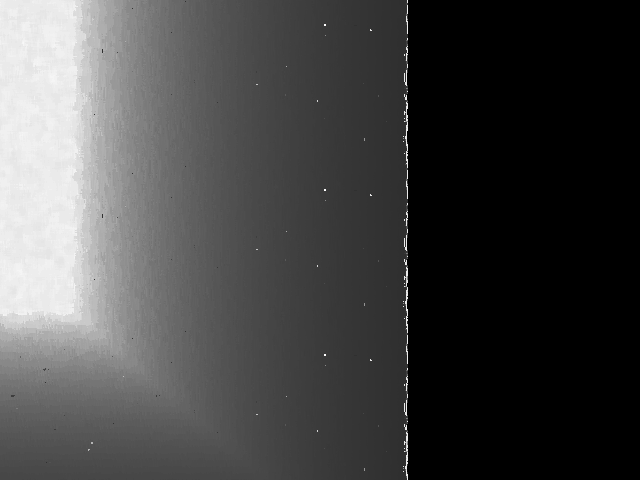
\includegraphics[width=2.5in]{imgs/Wall/depth.png}
    \caption{Depth map for the wall scenario.}
    \label{fig:wall_depth}
\end{figure}

\begin{figure}[!t]
    \centering
    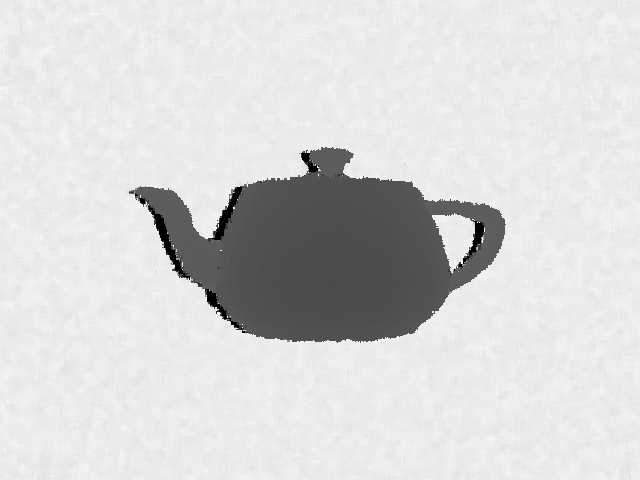
\includegraphics[width=2.5in]{imgs/Teapod/depth.png}
    \caption{Depth map for the teapot scenario.}
    \label{fig:teapot_depth}
\end{figure}

\begin{figure}[!t]
    \centering
    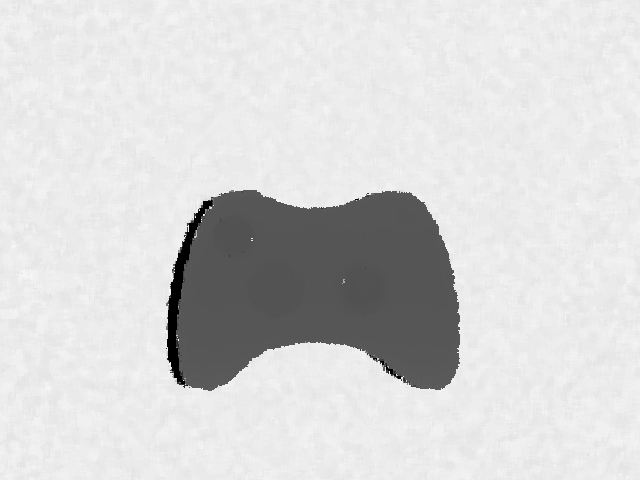
\includegraphics[width=2.5in]{imgs/XboxController/depth.png}
    \caption{Depth map for the Xbox controller scenario.}
    \label{fig:xbox_depth}
\end{figure}

With the resultant depth maps, the conversion to point cloud was achieved using the Open3D \cite{Zhou2018} library. In essence, this library applies equations \ref{eq:pointcloud_x} and \ref{eq:pointcloud_y} to compute the $x$ and $y$ coordinates and directly uses the depth map values as the $z$ coordinate. In our application, we computed the intrinsic parameters of the \gls{cmos} sensor as
% [[fx, 0, cx], [0, fy, cy], [0, 0, 1]]
\begin{equation*}
    \begin{bmatrix}
        f_x & 0 & c_x \\
        0 & f_y & c_y \\
        0 & 0 & 1
    \end{bmatrix}  
    %
    =
    %
    \begin{bmatrix}
        \frac{640}{\tan(FOV_x / 2)} & 0 & 640/2 \\
        0 & \frac{480}{\tan(FOV_y / 2)} & 480/2 \\
        0 & 0 & 1
    \end{bmatrix}  
    .
\end{equation*}

The correspondent point clouds are shown on figures \ref{fig:wall_pc}, \ref{fig:teapot_pc} and \ref{fig:xbox_pc}.

\begin{figure}[!t]
    \centering
    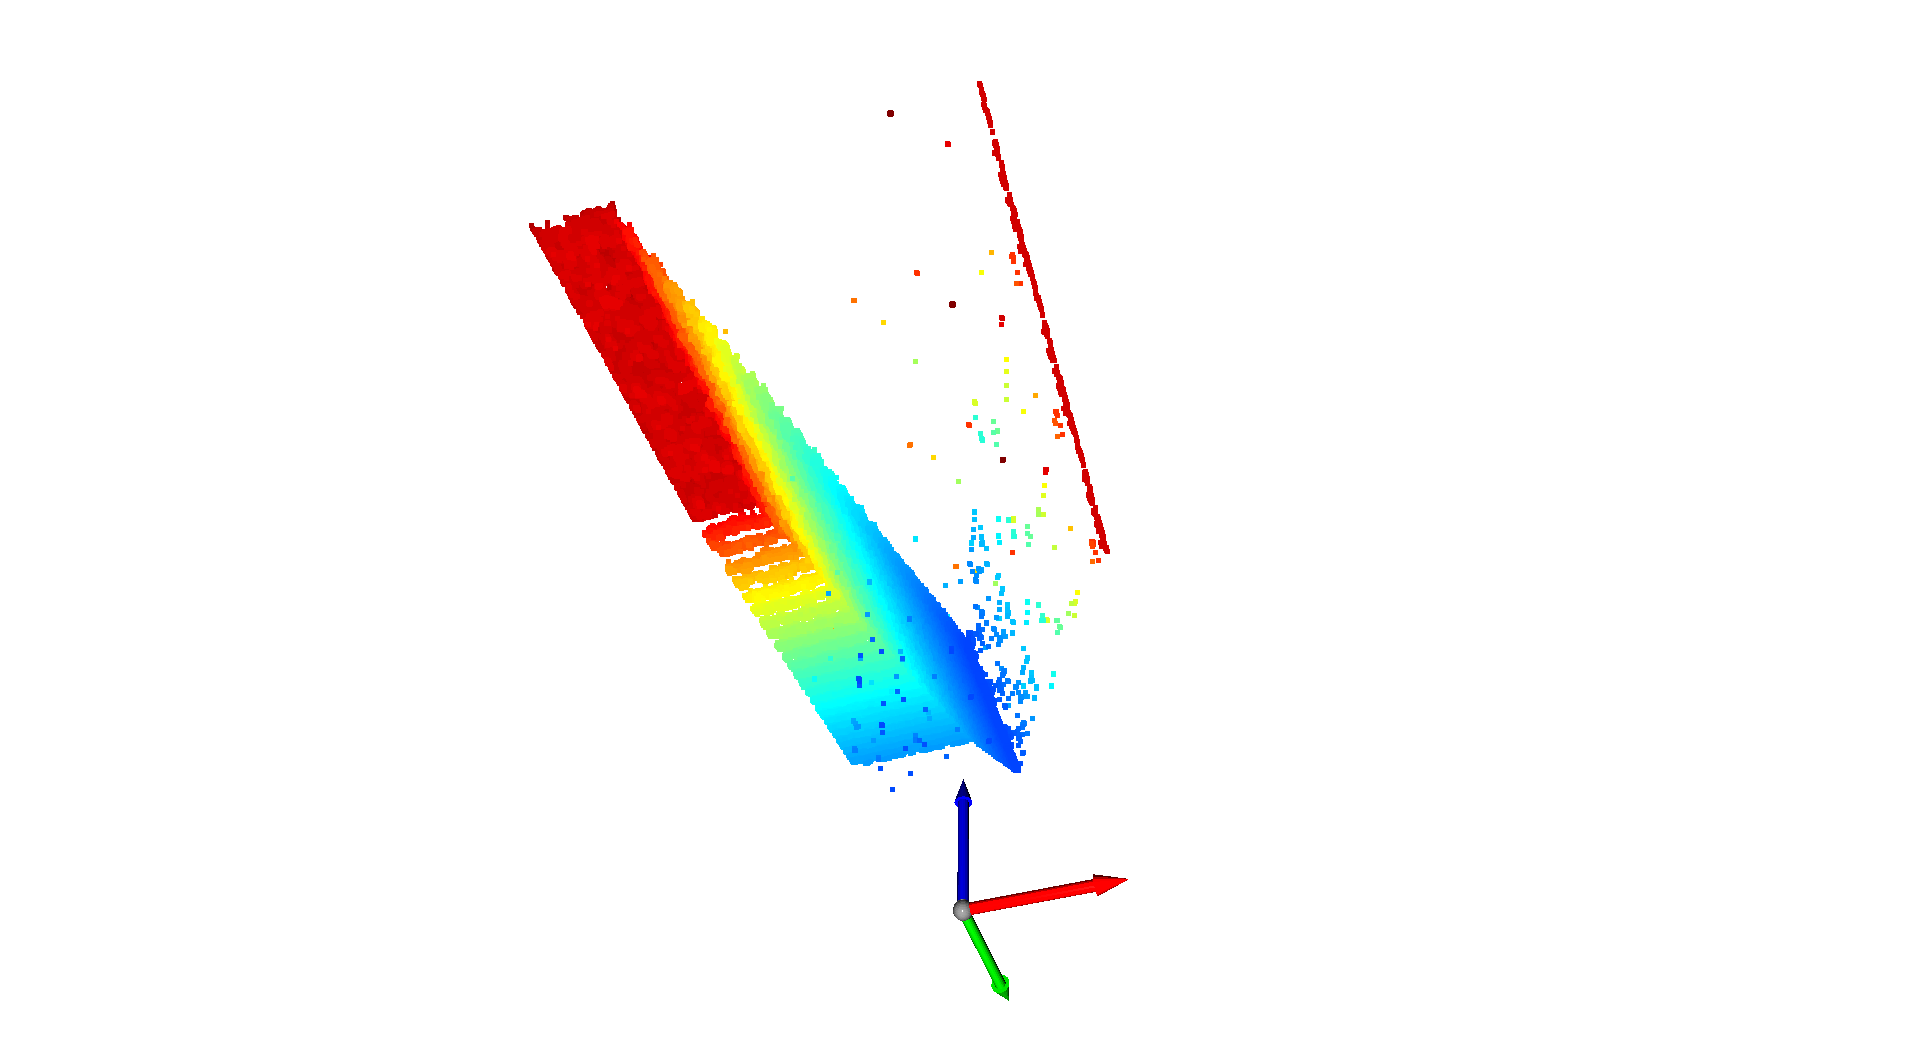
\includegraphics[width=2.5in]{imgs/Wall/pc.png}
    \caption{Point cloud for the wall scenario.}
    \label{fig:wall_pc}
\end{figure}

\begin{figure}[!t]
    \centering
    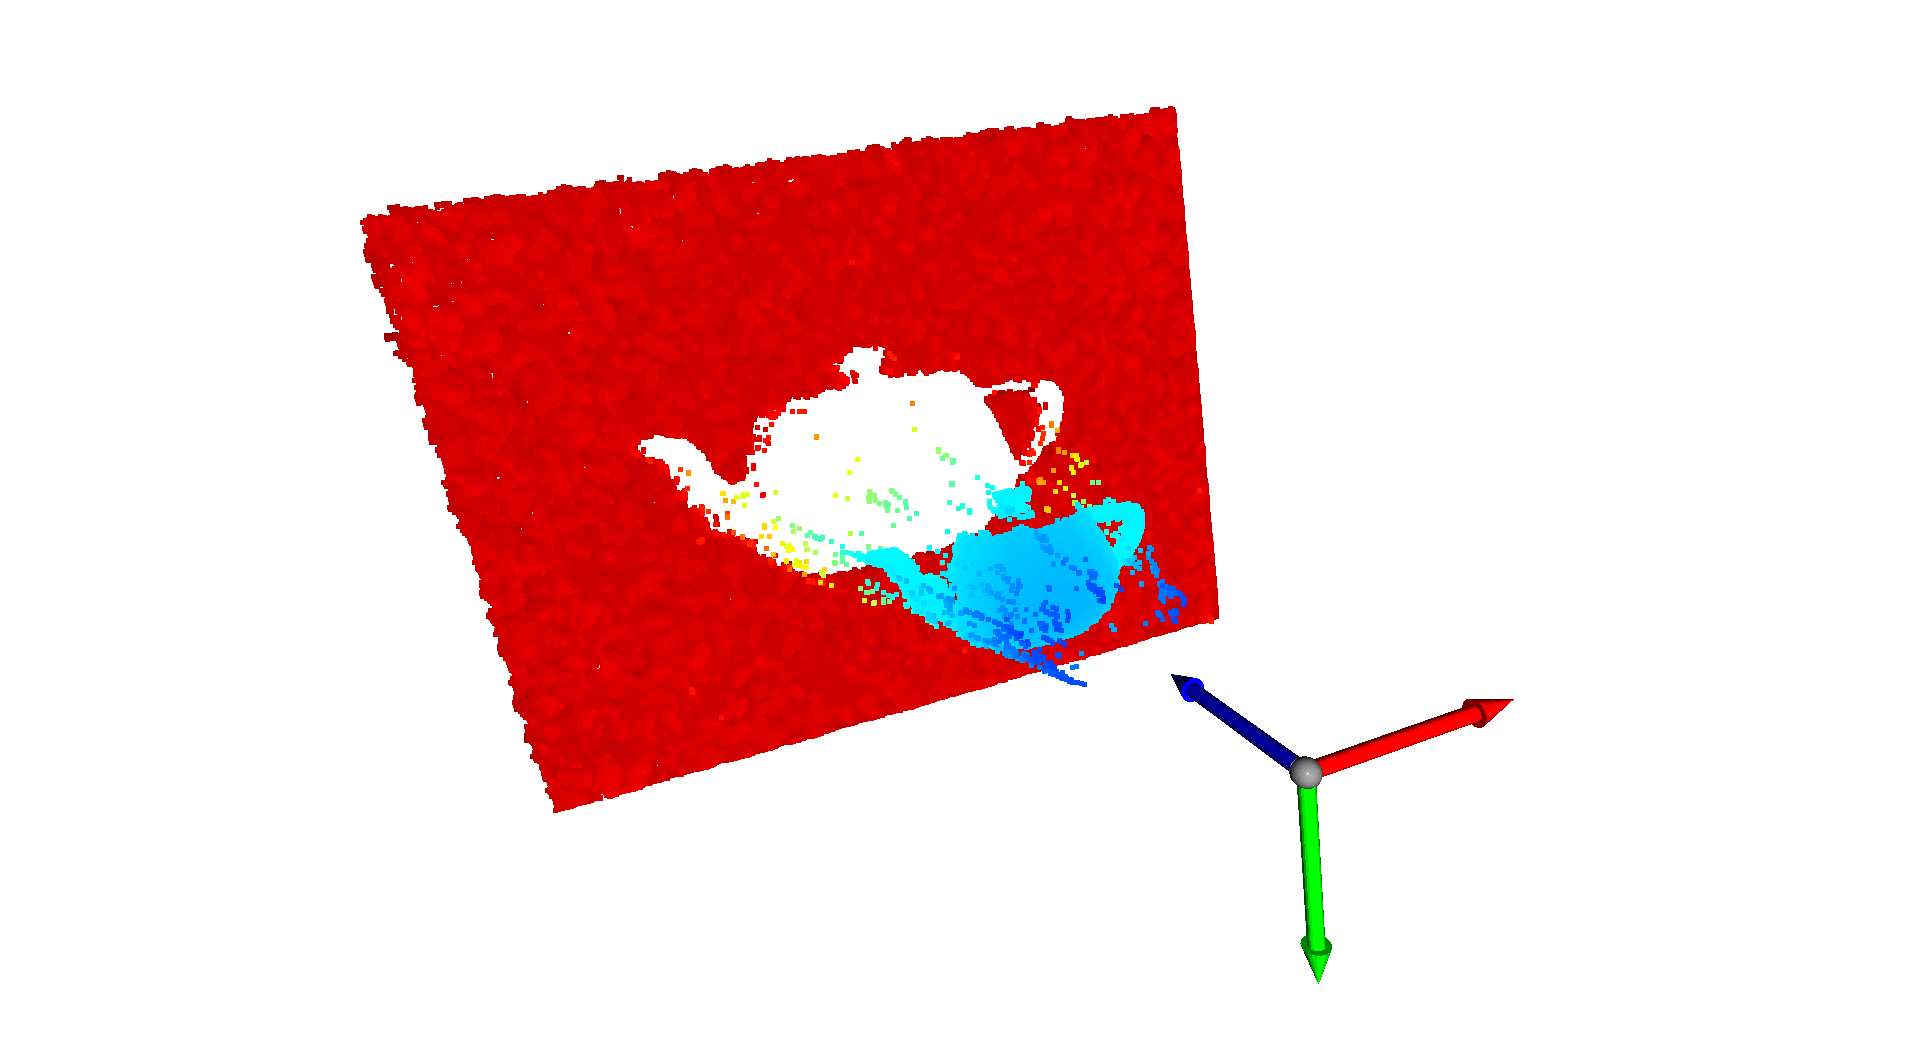
\includegraphics[width=2.5in]{imgs/Teapod/pc.png}
    \caption{Point cloud for the teapot scenario.}
    \label{fig:teapot_pc}
\end{figure}

\begin{figure}[!t]
    \centering
    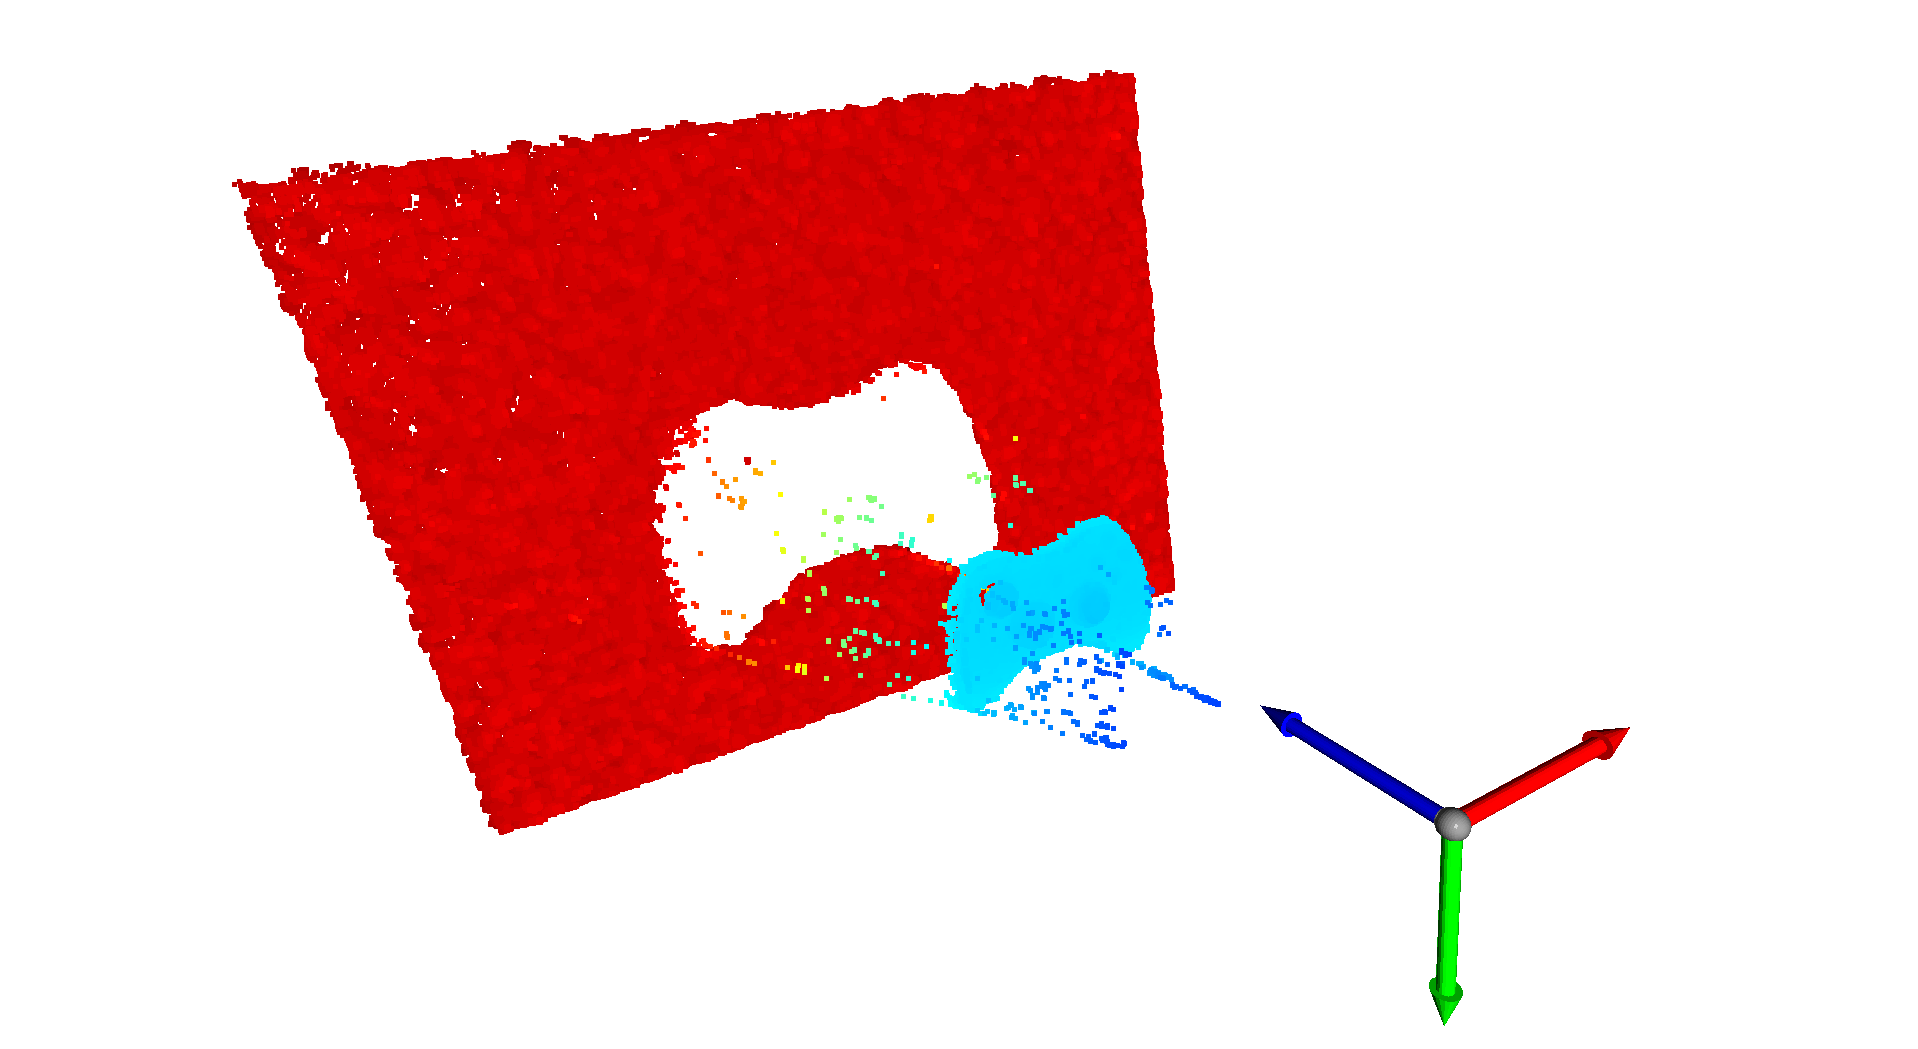
\includegraphics[width=2.5in]{imgs/XboxController/pc.png}
    \caption{Point cloud for the Xbox controller scenario.}
    \label{fig:xbox_pc}
\end{figure}

\subsection{Kinect Data}

After being successful at using the simulated \gls{ir} images to compute depth maps and, then, point clouds, the subsequent step was to acquire and handle the real data provided by a real Kinect. As an example, figure \ref{fig:kinect_frame} shows a frame, at the same instant, gathered from the video, depth and \gls{ir} streams.

\begin{figure*}[!t]
    \centering
        \subfloat[]{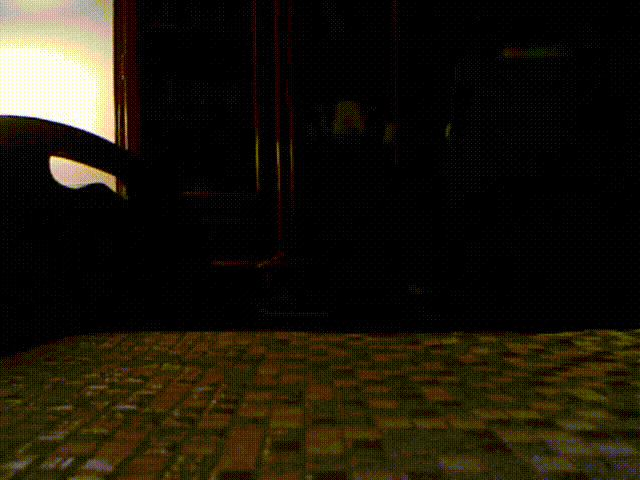
\includegraphics[width=2.5in]{imgs/Kinect/rgb.png}%
        \label{fig:kinect_frame_rgb}}
        \hfil
        \subfloat[]{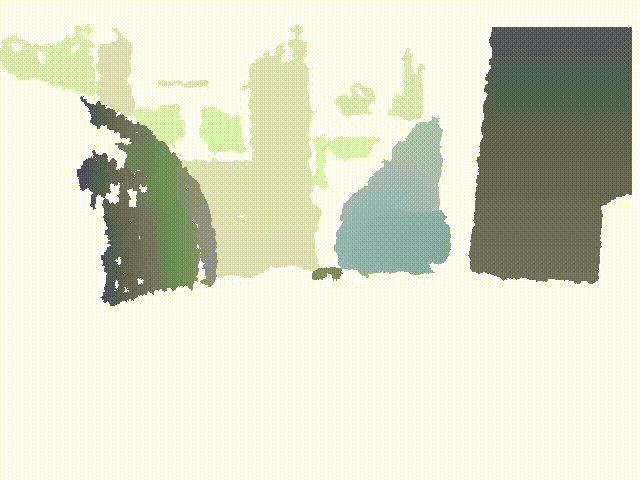
\includegraphics[width=2.5in]{imgs/Kinect/depth.png}%
        \label{fig:kinect_frame_depth}}
        \hfil
        \subfloat[]{
\includegraphics[width=2.5in]{imgs/Kinect/ir.png}%
        \label{fig:kinect_frame_ir}}
    \caption{A frame from the (a) video, (b) depth and (c) infrared streams captured at the same instant from a real Kinect.}
    \label{fig:kinect_frame}
\end{figure*}

Unfortunately, we could not integrate this images onto the depth estimation process. As show by figure \ref{fig:kinect_frame_ir}, much light coming from outside sources severely hinders the binarization of the speckle pattern. This was, as shown earlier, mandatory for the procedure to work.

\section{Future Work}

As guidelines for a future work, two main points can be quite improved.

The main point is the completion of the proposed goal, integrating the depth algorithm with the real Kinect data. This poses two main difficulties, i) study if the speckle pattern provided by \cite{landau2016kinect} actually reassembles close enough the actually projected pattern and ii) build a sufficiently robust binarization algorithm for the \gls{ir} images so that most of the non-pattern portions of the received image are filtered out. 

The secondary point should be to improve performance of the implementation. For reasonably small $640 \times 480$ images the algorithm is quite slow and would be unusable if applied to a commercial product. One proposal is to use a region growing algorithm and test if this actually produces satisfactory results with reduced computation time.



\section{Conclusion}

Although the the goal of building a fully functional, real-time, 3D structured light system was not reached, the authors believe that the current project builds the foundation for future works to accomplish it.

This work not only researched and resumed the essence of how the Kinect (and possible other camera systems based on the PrimeSense technology like the Asus Xtion, Orbec Astra, etc.) work but also proved to be possible the direct acquisition of \gls{ir} images.




% if have a single appendix:
%\appendix[Proof of the Zonklar Equations]
% or
%\appendix  % for no appendix heading
% do not use \section anymore after \appendix, only \section*
% is possibly needed

% use appendices with more than one appendix
% then use \section to start each appendix
% you must declare a \section before using any
% \subsection or using \label (\appendices by itself
% starts a section numbered zero.)
%


% \appendices
% \section{Proof of the First Zonklar Equation}
% Appendix one text goes here.

% you can choose not to have a title for an appendix
% if you want by leaving the argument blank
% \section{}
% Appendix two text goes here.


% use section* for acknowledgment
% \section*{Acknowledgment}


% The authors would like to thank...


% Can use something like this to put references on a page
% by themselves when using endfloat and the captionsoff option.
\ifCLASSOPTIONcaptionsoff
  \newpage
\fi



% trigger a \newpage just before the given reference
% number - used to balance the columns on the last page
% adjust value as needed - may need to be readjusted if
% the document is modified later
%\IEEEtriggeratref{8}
% The "triggered" command can be changed if desired:
%\IEEEtriggercmd{\enlargethispage{-5in}}

% references section

% can use a bibliography generated by BibTeX as a .bbl file
% BibTeX documentation can be easily obtained at:
% http://mirror.ctan.org/biblio/bibtex/contrib/doc/
% The IEEEtran BibTeX style support page is at:
% http://www.michaelshell.org/tex/ieeetran/bibtex/
\bibliographystyle{IEEEtran}
% argument is your BibTeX string definitions and bibliography database(s)
\bibliography{IEEEabrv, bib}
%
% <OR> manually copy in the resultant .bbl file
% set second argument of \begin to the number of references
% (used to reserve space for the reference number labels box)
% \begin{THEBibliography}{1}

% \bibitem{IEEEhowto:kopka}
% H.~Kopka and P.~W. Daly, \emph{A Guide to \LaTeX}, 3rd~ed.\hskip 1em plus
%   0.5em minus 0.4em\relax Harlow, England: Addison-Wesley, 1999.

% \end{thebibliography}

% biography section
% 
% If you have an EPS/PDF photo (graphicx package needed) extra braces are
% needed around the contents of the optional argument to biography to prevent
% the LaTeX parser from getting confused when it sees the complicated
% \includegraphics command within an optional argument. (You could create
% your own custom macro containing the \includegraphics command to make things
% simpler here.)
%\begin{IEEEbiography}[{\includegraphics[width=1in,height=1.25in,clip,keepaspectratio]{mshell}}]{Michael Shell}
% or if you just want to reserve a space for a photo:

% \begin{IEEEbiography}{Michael Shell}
% Biography text here.
% \end{IEEEbiography}

% if you will not have a photo at all:
% \begin{IEEEbiographynophoto}{John Doe}
% Biography text here.
% \end{IEEEbiographynophoto}

% insert where needed to balance the two columns on the last page with
% biographies
%\newpage

% \begin{IEEEbiographynophoto}{Jane Doe}
% Biography text here.
% \end{IEEEbiographynophoto}

% You can push biographies down or up by placing
% a \vfill before or after them. The appropriate
% use of \vfill depends on what kind of text is
% on the last page and whether or not the columns
% are being equalized.

%\vfill

% Can be used to pull up biographies so that the bottom of the last one
% is flush with the other column.
%\enlargethispage{-5in}



% that's all folks
\end{document}


